\documentclass[tikz,border=2pt]{standalone}
\usepackage{amsmath,amssymb}
\begin{document}
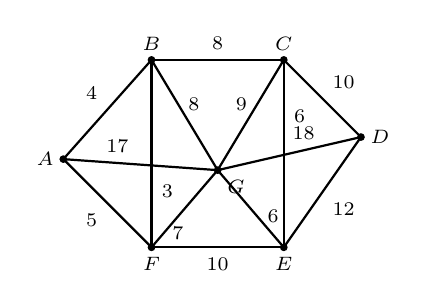
\begin{tikzpicture}[scale=0.7, font=\scriptsize]
	\coordinate (A) at (-2.6,0);
	\coordinate (B) at (-1,1.8);
	\coordinate (C) at (1.4,1.8);
	\coordinate (D) at (2.8,0.4);
	\coordinate (E) at (1.4,-1.6);
	\coordinate (F) at (-1,-1.6);
	\coordinate (G) at (0.2,-0.2);
	
	\draw[thick] (A)--(B) node[midway,above left] {$4$};
	\draw[thick] (B)--(C) node[midway,above] {$8$};
	\draw[thick] (C)--(D) node[midway,above right] {$10$};
	\draw[thick] (D)--(E) node[midway,below right] {$12$};
	\draw[thick] (E)--(F) node[midway,below] {$10$};
	\draw[thick] (F)--(A) node[midway,below left] {$5$};
	
	\draw[thick] (A)--(G) node[pos=0.35,above] {$17$};
	\draw[thick] (B)--(G) node[pos=0.4,right] {$8$};
	\draw[thick] (C)--(G) node[pos=0.4,left] {$9$};
	\draw[thick] (D)--(G) node[pos=0.4,above] {$18$};
	\draw[thick] (E)--(G) node[pos=0.4,right] {$6$};
	\draw[thick] (F)--(G) node[pos=0.4,below] {$7$};
	\draw[thick] (B)--(F) node[pos=0.7,right] {$3$};
	\draw[thick] (C)--(E) node[pos=0.3,right] {$6$};
	
	\foreach \p/\l/\pos in {A/A/left, B/B/above, C/C/above, D/D/right, E/E/below, F/F/below, G/G/below right} {
		\fill (\p) circle (2pt);
		\node[\pos] at (\p) {$\l$};
	}
\end{tikzpicture}
\end{document}
